\section{Introduction}
In recent years,the Internet of Things (IoT) has gathered significant traction which has led
to the exponential increase in the number of devices connected to the internet. %IoT involves the connection of heterogeneous devices with sensing and actuating capabilities over the internet. 
It has revolutionized devices to device communication, which in turn optimizes efficiency and improves the standard of living. According to a report released by Cisco, it is estimated that a total of 50 million devices will be connected to the internet by the year 2020.  With the vast amounts of connected heterogeneous devices, security and privacy risks are increased. Data provenance is instrumental to the security IoT data. Provenance describes a holistic history of operations  performed on a data object from its point of creation. Provenance can be used as a measure to ensure trust and also for forensic analysis in an event of malicious attack. Provenance collection system is of immense benefit to IoT devices however provenance incurs additional storage overhead. Continuous provenance collection has the tendency to generate more data than the data it describes. Work done by Brian et al demonstrates that changes to a source file in the Linux kernel results to two kilobytes of additional provenance data when the kernel is recompiled. Additionally, Figure x displays a graph of the growth of provenance data for a raspberry pi collecting temperature and humidity readings. This sensor reading is stored in CTF format. From the diagram we can see that the data grows rapidly with time. This motivates the need for an efficient pruning technique to reduce storage overhead that might be incurred by including provenance in an IoT application. It is of utmost importance to provide a method of pruning provenance data generated thereby reducing the storage overhead. This requirement is further motivated by the constrained memory and computing power of IoT devices. Pruning can be described as removing provenance data in order to conserve storage. 
 \par In this paper, we propose a fine-grained, policy model for provenance pruning. This model provides an expressive policy language which allows device administrators the flexibility of specifying what provenance data to store.  We argue that policy is an effective way of addressing the data pruning problem created by automatic provenance collection. With access control, we allow the flexibility of deciding what provenance data is discarded thereby eliminating unwanted provenance information. Provenance sometimes generates information that might be considered uninteresting. For example, a system collecting the provenance of system events such as device internal system state might be considered uninteresting to a researcher working on collecting temperature and humidity readings or a device administrator interested on. We implement a proof of concept system using XACML, a fine-grained attribute based access control policy language which evaluates request based on a policy specifications. XACML serves as the foundation for our framework.We compared our performance of the proposed framework with state of the art on provenance pruning (e.g web compression + dictionary). The remaining portion of the paper is outlined as follows: Section 2 discusses background information on IoT provenance pruning. Section 3 talks about related work on provenance pruning. Section 4 discusses implementation techniques, section 5 talks discusses experimental evaluation and finally, section 6 concludes and discusses future works.







IoT trace is derived in the form of CTF output. This output stream is pruned to reduce storage overhead.

CTF is a binary format that allows dynamic instrumentation trace of a applications written in C/C++. The source code for applications  is compiled with the generated c code that barectf creates for the IoT trace event. 

barectf is chosen for tracing IoT device because it generates ANCI C code which is lightweight and can fit into most microcontrollers.

%This mode can also the further applied for access control on resources in an IoT.
%
%Sensor based access control model for authentication and enforcement of provenance data.


%The \textit{proceedings} are the records of a conference\footnote{This
%  is a footnote}.  ACM seeks
%to give these conference by-products a uniform, high-quality
%appearance.  To do this, ACM has some rigid requirements for the
%format of the proceedings documents: there is a specified format
%(balanced double columns), a specified set of fonts (Arial or
%Helvetica and Times Roman) in certain specified sizes, a specified
%live area, centered on the page, specified size of margins, specified
%column width and gutter size.

\section{BACKGROUND}

This section describes key concepts of data provenance, IoT characteristics, and provenance models. It also provides motivating example for the need for provenance pruning.

\subsection{Internet of Things}
There is no standard definition for IoT, however, researchers have tried to define the concept
of connected \"things\". The concept of IoT was proposed by Mark Weiser in the early 1990s
 which represents a way in which the physical objects, \" things\", can be connected to the
digital world. Gubbi et al defines the IoT as an interconnection of sensing and actuating
devices that allows data sharing across platforms through a centralized framework. We
define (IoT) as follows:

\begin{definition}

The Internet of Things (IoT) is a network of heterogeneous devices with
sensing and actuating capabilities communicating over the internet.

\end{definition}


The notion of IoT has been attributed to smart devices. The interconnectivity between
various heterogeneous devices allows for devices to share information in a unique manner.
Analytics is a driving force for IoT. With analytics, devices can learn from user data
to make smarter decisions. This notion of smart devices is seen in various commercial
applications such as smartwatches, thermostats that automatically learns a user patterns. The ubiquitous nature of these devices make them ideal choices to be included in consumer products.  IoT architecture represents a functional hierarchy of how information is disseminated across
multiple hierarchies contained in an IoT framework; from devices which contain sensing and
actuating capabilities to massive data centers (cloud storage). Knowing how information
is transmitted across layers allows a better understanding on how to model the flow of
information across actors contained in an IoT hierarchy.
Figure 1 displays the IoT architecture and the interactions between the respective
layers. IoT architecture consists of four distinct layers: The sensor and actuator layer, device layer, gateway layer and the cloud layer. The base of the architectural stack consist of sensors and actuators which gathers provenance information and interacts with the device layer. The device layer consists of
devices (e.g mobile phones, laptops, smart devices) which are responsible for aggregating
data collected from sensors and actuators. These devices in turn forwards the aggregated
data to the gateway layer. The gateway layer routes and forwards data collected from the
device later. It could also serve as a medium of temporary storage and data processing.
The cloud layer is involved with the storage and processing of data collected from the
gateway layer. Note that the resource constraints decreases up the architectural stack with
the cloud layer having the most resources (memory, power computation) and the sensor-
actuator layer having the least.



Automatic provenance collection. For pruning in general, web compression and web compression + dictionary compression are techniques that has been effectively suggested in the literature. This techniques are considered efficient in pruning provenance but they fail to address the issue of pruning provenance data that might be uninteresting to the device administrator of an automatic provenance collection system. Motivated by the work of Brian et al suggests the need for a policy driven provenance collection system in which system events that are important to device administrator is collected thereby leaving out interesting events which increases storage overhead. While we consider pruning to be an effective way to address the issue of storage overhead, there exist a tradeoff between the data that is pruned and its importance to the collective provenance. To this end, we define a probabilistic model that estimates the risk involved in deleting unwanted provenance data. With is information, the user is left to decide if the provenance data in question that is deleted is considered important to the provenance chain. 


For provenance to be effective in forensic analysis, it has to be complete   





\begin{figure}[h]
\begin{center}

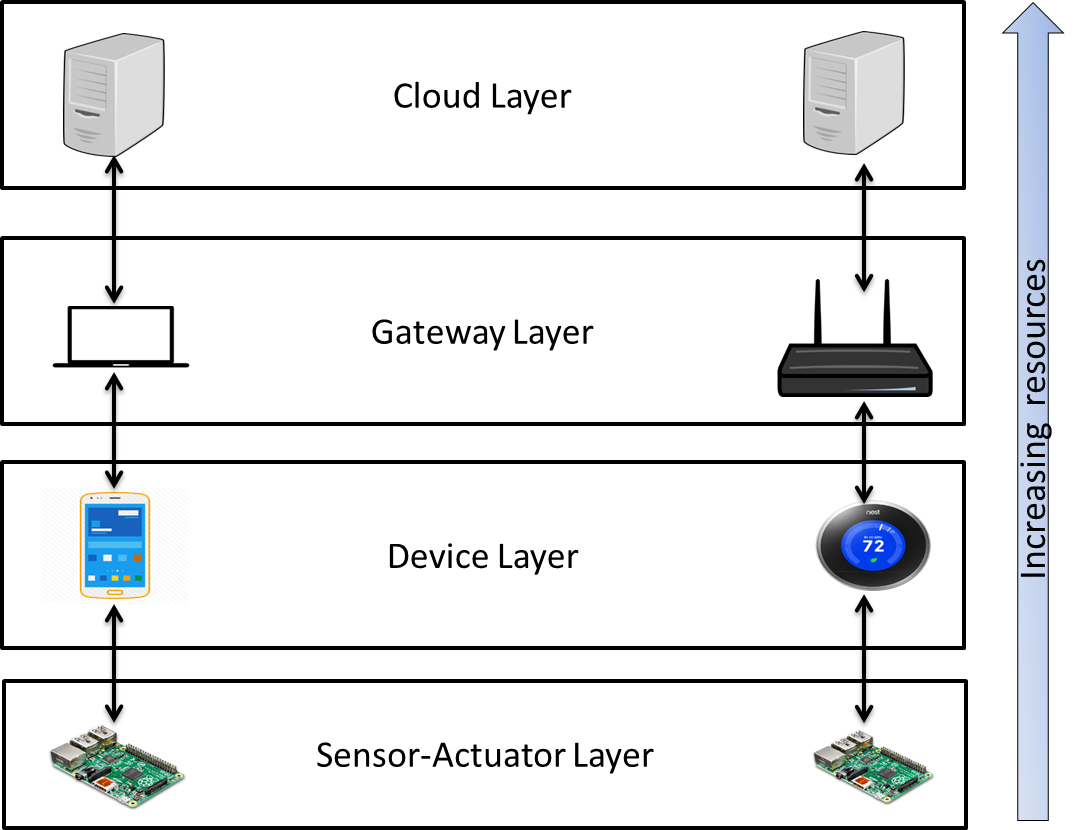
\includegraphics[height=2.0in]{iot_architecture.png}
\end{center}
\caption{IoT Architecture Diagram. The arrows illustrates the interaction between data at various layers on the architecture.}
\label{iot_architecture}

\end{figure}




With the recent data explosion [22] due to the large influx  in amounts of interconnected devices, information is disseminated at a fast rate and with this increase involves security and privacy concerns. Creating a provenance-aware system is beneficial to IoT because it
ensures the trust and integrity of interconnected devices. Enabling provenance collection in IoT devices allows these devices to capture valuable information which enables backtracking
in an event of a malicious attack. 





\subsection{Data Provenance}

The Oxford English dictionary defines provenance as the place of origin or earliest
known history of something". An example of provenance can be seen with a college transcript. A transcript is the provenance of a college degree because it outlines all of the
courses satisfied in order to attain the degree. In the field of computing, data provenance, also known as data lineage, can be defined
as the history of all activities performed on entities from its creation to its current state.
Cheney et al.  decribes provenance as the origin and history of data from its lifecycle. Buneman et al describes provenance from a database perspective as the origin of data and the steps in which it is derived in the database system. We formally define provenance as follows: 

\begin{definition}
Data provenance of an entity is a comprehensive history of activities that occur on that entity from its creation to its present state.
\end{definition}

\par Provenance ensures trust and integrity of data \cite{Bertino2015}. It outlines causality and dependency between all objects involved in the system and allows for the verification of the source of data. Causality and dependency are used to determine the relationship between multiple objects. The relationship in which provenance denotes can in turn be used in digital forensics \cite{zawoadfecloud} to investigate the cause of a malicious attack and also in intrusion detection systems to further enhance the security of computing devices. 
 



%\subsection{Provenance-system collection}
%
%\subsubsection{Observed Provenance}
%
%\subsubsection{Disclosed Provenance}



\subsection{Provenance Characteristics}

Since provenance denotes the who, where and why of data transformation, it is imperative that data disseminated in an IoT architecture satisfies the required conditions. The characteristics of data provenance are outlined in detail below.


\begin{itemize}

\item Who: This characteristic provides information on activities made to an entity. Knowing the ``who" characteristic is essential because it maps the identity of modification to a particular data object. An example of ``who" in an IoT use case is a sensor device identifier.

\item Where: This characteristic denotes location information in which data transformation was made. This provenance characteristic could be optional since not every data modification contains location details.

\item When: This characteristic denotes the time information at which data transformation occurred. This is an essential provenance characteristic. Being able to tell the time of a data transformation allows for tracing data irregularities.

\item What: This characteristic denotes the transformation is applied on a data object. A use case for IoT can be seen in the various operations (create, read, update, and delete) that could be performed on a file object.

\end{itemize}


There are two ways of pruning Provenance data: Provenance can be pruned at collection before it is been committed to the disk  or after being recorded to disk. Policy defines rules and actions that should be taken if any of the rules applies.  Access control in this case is used as a tool for pruning provenance data stored on an IoT device. It can also be extended for traditional access control measures. Data pruning is an essential problem for automatic provenance collection. Observed provenance and disclosed provenance. Observed provenance involves automatic collection of system states and changes. One major drawback of this method is that all system events are provenanced including irrelevant system provenance which incurs more storage overhead. Described provenance on the other hand, allows a user to provide a workflow of how what provenance the system is intended to generate and an engine to execute the workflow described.

\section{System Model}

We have already seen several typeface changes in this sample.  You can
indicate italicized words or phrases in your text with the command
\texttt{{\char'134}textit}; emboldening with the command
\texttt{{\char'134}textbf} and typewriter-style (for instance, for
computer code) with \texttt{{\char'134}texttt}.  But remember, you do
not have to indicate typestyle changes when such changes are part of
the \textit{structural} elements of your article; for instance, the
heading of this subsection will be in a sans serif\footnote{Another
  footnote, here.  Let's make this a rather short one to see how it
  looks.} typeface, but that is handled by the document class file.
Take care with the use of\footnote{A third, and last, footnote.}  the
curly braces in typeface changes; they mark the beginning and end of
the text that is to be in the different typeface.

You can use whatever symbols, accented characters, or non-English
characters you need anywhere in your document; you can find a complete
list of what is available in the \textit{\LaTeX\ User's Guide}
\cite{Lamport:LaTeX}.

\subsection{Data Model}
 Provenance data is collected using dynamic instrumentation by attaching barectf trace endpoints to dynamically generate CTF trace. This information is stored on the IoT device. Provenance trace is  Sensor  and actuator reading is represented as a tuple $<ts, [r_1,r_2,...,r_n]>$ where $ts$ is denoted as the timestamp and $r_1,...r_n$ denotes the various data points from the sensor readings. Access control is enforced using a modified version of the  security punctuations model.


The policy language is flexible and written in a way that is easily understood. Policy specifies the appropriate groups for each sensor readings. Every sensor attribute is grouped. For each group, there exist and associated role For each role, there is an action of permit or deny. The user who serves as the device administrator is in charge of  appropriate sensor data groups. This information is combined to provide permit or deny decisions.  This policy with the appropriate request is evaluated to produce appropriate access decision.


Let G be a sensor group and R represents user roles, and U represent



For pruning, access control is used to determine if provenance data should be stored on the device or not this way, data that is discarded is considered invaluable to the organization.


Parts of provenance in which data is deleted can also be marked as deleted theryby maintaining the provenance chain. Data deleted can also be marked. A hybrid apporach which emplys policy and compression can also be implemented. 




For example, a research scientist requires temperature/humidity data for research on the environmental outcome over time. He tries to collects temperature and humidity readings of the environment using a raspberry pi and temp/humidity sensor. The sensor readings and relationship between other sensor readings forms the basis of provenanc. provenance is collected from the sensor and stored on the raspberry pi. The device administrator in this case is the scientist performing the experiment. They decide that they only want to store all temperature from a certain time interval. Also, they set a storage threshold, which after this provenance data is automatically discarded. 

We also calculate 
\subsubsection{Access Control Model}
A formula that appears in the running text is called an
inline or in-text formula.  It is produced by the
\textbf{math} environment, which can be
invoked with the usual \texttt{{\char'134}begin\,\ldots{\char'134}end}
construction or with the short form \texttt{\$\,\ldots\$}. You
can use any of the symbols and structures,
from $\alpha$ to $\omega$, available in
\LaTeX~\cite{Lamport:LaTeX}; this section will simply show a
few examples of in-text equations in context. Notice how
this equation:
\begin{math}
  \lim_{n\rightarrow \infty}x=0
\end{math},
set here in in-line math style, looks slightly different when
set in display style.  (See next section).

\subsubsection{Display Equations}
A numbered display equation---one set off by vertical space from the
text and centered horizontally---is produced by the \textbf{equation}
environment. An unnumbered display equation is produced by the
\textbf{displaymath} environment.

Again, in either environment, you can use any of the symbols
and structures available in \LaTeX\@; this section will just
give a couple of examples of display equations in context.
First, consider the equation, shown as an inline equation above:
\begin{equation}
  \lim_{n\rightarrow \infty}x=0
\end{equation}
Notice how it is formatted somewhat differently in
the \textbf{displaymath}
environment.  Now, we'll enter an unnumbered equation:
\begin{displaymath}
  \sum_{i=0}^{\infty} x + 1
\end{displaymath}
and follow it with another numbered equation:
\begin{equation}
  \sum_{i=0}^{\infty}x_i=\int_{0}^{\pi+2} f
\end{equation}
just to demonstrate \LaTeX's able handling of numbering.


\section{proposed Model}
The policy framework consists of a policy engine. The policy engine contains authorization and enforcement components that provides and enforce decisions on how provenance data should be stored. A policy document is a component of the policy framework. It identifies provenance data that is considered relevant to the IoT application. Our policy architecture is modeled using the Common Open Policy Service (COPS) Standard \cite{rfc2748}. COPS consists of components for policy generation, evaluation and enforcement. The Policy Enforcement Point (PEP) enforces decisions received from the Policy Decision Point (PDP). The PDP evaluates policies and generates decision based on the evaluation. The model can be extended to include a secondary decision point (SDP) which allows for distributed policy evaluation, thus freeing up the PDP from communication bottlenecks caused by large amounts of requests received by a single PDP. Figure \ref{policy_architecture} below illustrates the system architecture of our proposed policy-based storage framework. Different layers of the IoT architecture contain different decision and enforcement components. The sensor-actuator layer of the IoT architecture is omitted because it has negligible memory resources and the  sensors and actuators are usually physically part of a device in the device layer and as such does not have any data to prune. 


Policy document which is generated by the policy creator serves as an input to the PDP component and is evaluated at the device, gateway and cloud layer. The PEP which is involved with generating requests is located in the device and gateway layer. SDPs can be located in the gateway layer, which allows for policy evaluation without incurring additional network overhead of communicating with the PDP located in the cloud layer. 




%% you removed the XACML section from here.

\par Using the use case of the smart home depicted in chapter 2, a policy framework could be implemented and incorporated into the IoT architecture which allows a device administrators to specify what kinds of provenance data to collect. The policy acts an enforcement point providing an efficient storage mechanism in a resource constrained environment. 

%The contents of the implementation details for the policy framework which specifies the policy grammar and the policy architecture across the IoT stack are left as future work.

\begin{figure}[ht!]
\begin{center}
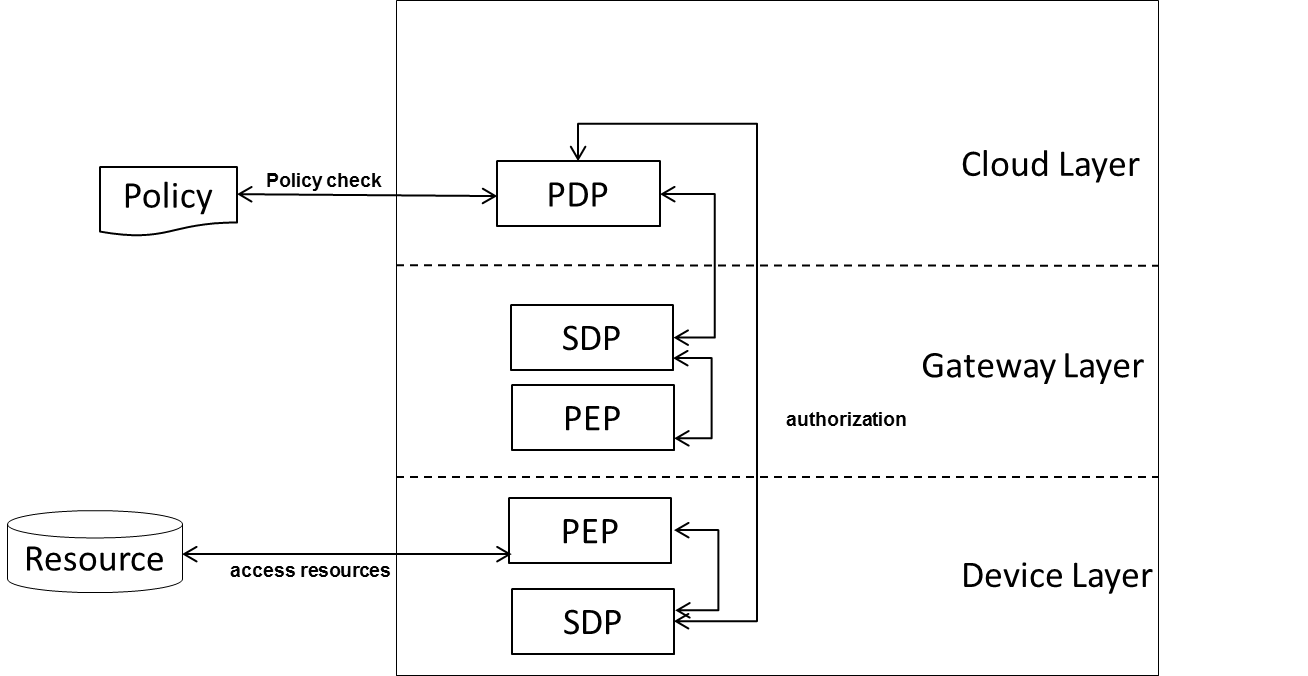
\includegraphics[height=2.0in]{policy.png}
\caption{Policy based system architecture which allows for effective storage of provenance data}
\label{policy_architecture}
\end{center}
\end{figure}


\section{Experiment}


\section{Related Work}

Bates et al proposed a framework, provenance wall. Provenance wall uses Mandatory Access Control in which every system object is assigned a security label. The MAC contains a policies which determines permissible actions of security labels. MAC labels are placed as an overlay to Provenance objects. This way, only the provenance information that are contained in the MAC policy is permitted to be stored.  Xie et al proposes using web compression techniques for provenance punning. Since provenance can be represented as graph and has similarities to a web graph. They achieve this process by encoding similar successor list from the previous node in an adjacency matrix, encoding successive number by recording the start, finally encoding number of gaps between successor nodes rather than the successor itself.

\subsection{Citations}
Citations to articles~\cite{bowman:reasoning,
clark:pct, braams:babel, herlihy:methodology},
conference proceedings~\cite{clark:pct} or maybe
books \cite{Lamport:LaTeX, salas:calculus} listed
in the Bibliography section of your
article will occur throughout the text of your article.
You should use BibTeX to automatically produce this bibliography;
you simply need to insert one of several citation commands with
a key of the item cited in the proper location in
the \texttt{.tex} file~\cite{Lamport:LaTeX}.
The key is a short reference you invent to uniquely
identify each work; in this sample document, the key is
the first author's surname and a
word from the title.  This identifying key is included
with each item in the \texttt{.bib} file for your article.

The details of the construction of the \texttt{.bib} file
are beyond the scope of this sample document, but more
information can be found in the \textit{Author's Guide},
and exhaustive details in the \textit{\LaTeX\ User's
Guide} by Lamport~\shortcite{Lamport:LaTeX}.


This article shows only the plainest form
of the citation command, using \texttt{{\char'134}cite}.

\subsection{Tables}
Because tables cannot be split across pages, the best
placement for them is typically the top of the page
nearest their initial cite.  To
ensure this proper ``floating'' placement of tables, use the
environment \textbf{table} to enclose the table's contents and
the table caption.  The contents of the table itself must go
in the \textbf{tabular} environment, to
be aligned properly in rows and columns, with the desired
horizontal and vertical rules.  Again, detailed instructions
on \textbf{tabular} material
are found in the \textit{\LaTeX\ User's Guide}.

Immediately following this sentence is the point at which
Table~\ref{tab:freq} is included in the input file; compare the
placement of the table here with the table in the printed
output of this document.

\begin{table}
  \caption{Frequency of Special Characters}
  \label{tab:freq}
  \begin{tabular}{ccl}
    \toprule
    Non-English or Math&Frequency&Comments\\
    \midrule
    \O & 1 in 1,000& For Swedish names\\
    $\pi$ & 1 in 5& Common in math\\
    \$ & 4 in 5 & Used in business\\
    $\Psi^2_1$ & 1 in 40,000& Unexplained usage\\
  \bottomrule
\end{tabular}
\end{table}

To set a wider table, which takes up the whole width of the page's
live area, use the environment \textbf{table*} to enclose the table's
contents and the table caption.  As with a single-column table, this
wide table will ``float'' to a location deemed more desirable.
Immediately following this sentence is the point at which
Table~\ref{tab:commands} is included in the input file; again, it is
instructive to compare the placement of the table here with the table
in the printed output of this document.


\begin{table*}
  \caption{Some Typical Commands}
  \label{tab:commands}
  \begin{tabular}{ccl}
    \toprule
    Command &A Number & Comments\\
    \midrule
    \texttt{{\char'134}author} & 100& Author \\
    \texttt{{\char'134}table}& 300 & For tables\\
    \texttt{{\char'134}table*}& 400& For wider tables\\
    \bottomrule
  \end{tabular}
\end{table*}
% end the environment with {table*}, NOTE not {table}!

It is strongly recommended to use the package booktabs~\cite{Fear05}
and follow its main principles of typography with respect to tables:
\begin{enumerate}
\item Never, ever use vertical rules.
\item Never use double rules.
\end{enumerate}
It is also a good idea not to overuse horizontal rules.


\subsection{Figures}

Like tables, figures cannot be split across pages; the best placement
for them is typically the top or the bottom of the page nearest their
initial cite.  To ensure this proper ``floating'' placement of
figures, use the environment \textbf{figure} to enclose the figure and
its caption.

This sample document contains examples of \texttt{.eps} files to be
displayable with \LaTeX.  If you work with pdf\LaTeX, use files in the
\texttt{.pdf} format.  Note that most modern \TeX\ systems will convert
\texttt{.eps} to \texttt{.pdf} for you on the fly.  More details on
each of these are found in the \textit{Author's Guide}.

\begin{figure}
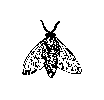
\includegraphics{fly}
\caption{A sample black and white graphic.}
\end{figure}

\begin{figure}
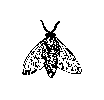
\includegraphics[height=1in, width=1in]{fly}
\caption{A sample black and white graphic
that has been resized with the \texttt{includegraphics} command.}
\end{figure}


As was the case with tables, you may want a figure that spans two
columns.  To do this, and still to ensure proper ``floating''
placement of tables, use the environment \textbf{figure*} to enclose
the figure and its caption.  And don't forget to end the environment
with \textbf{figure*}, not \textbf{figure}!

\begin{figure*}
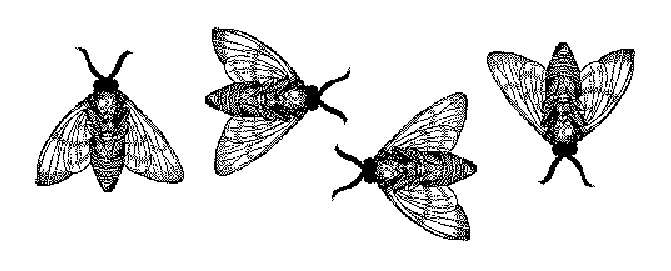
\includegraphics{flies}
\caption{A sample black and white graphic
that needs to span two columns of text.}
\end{figure*}


\begin{figure}
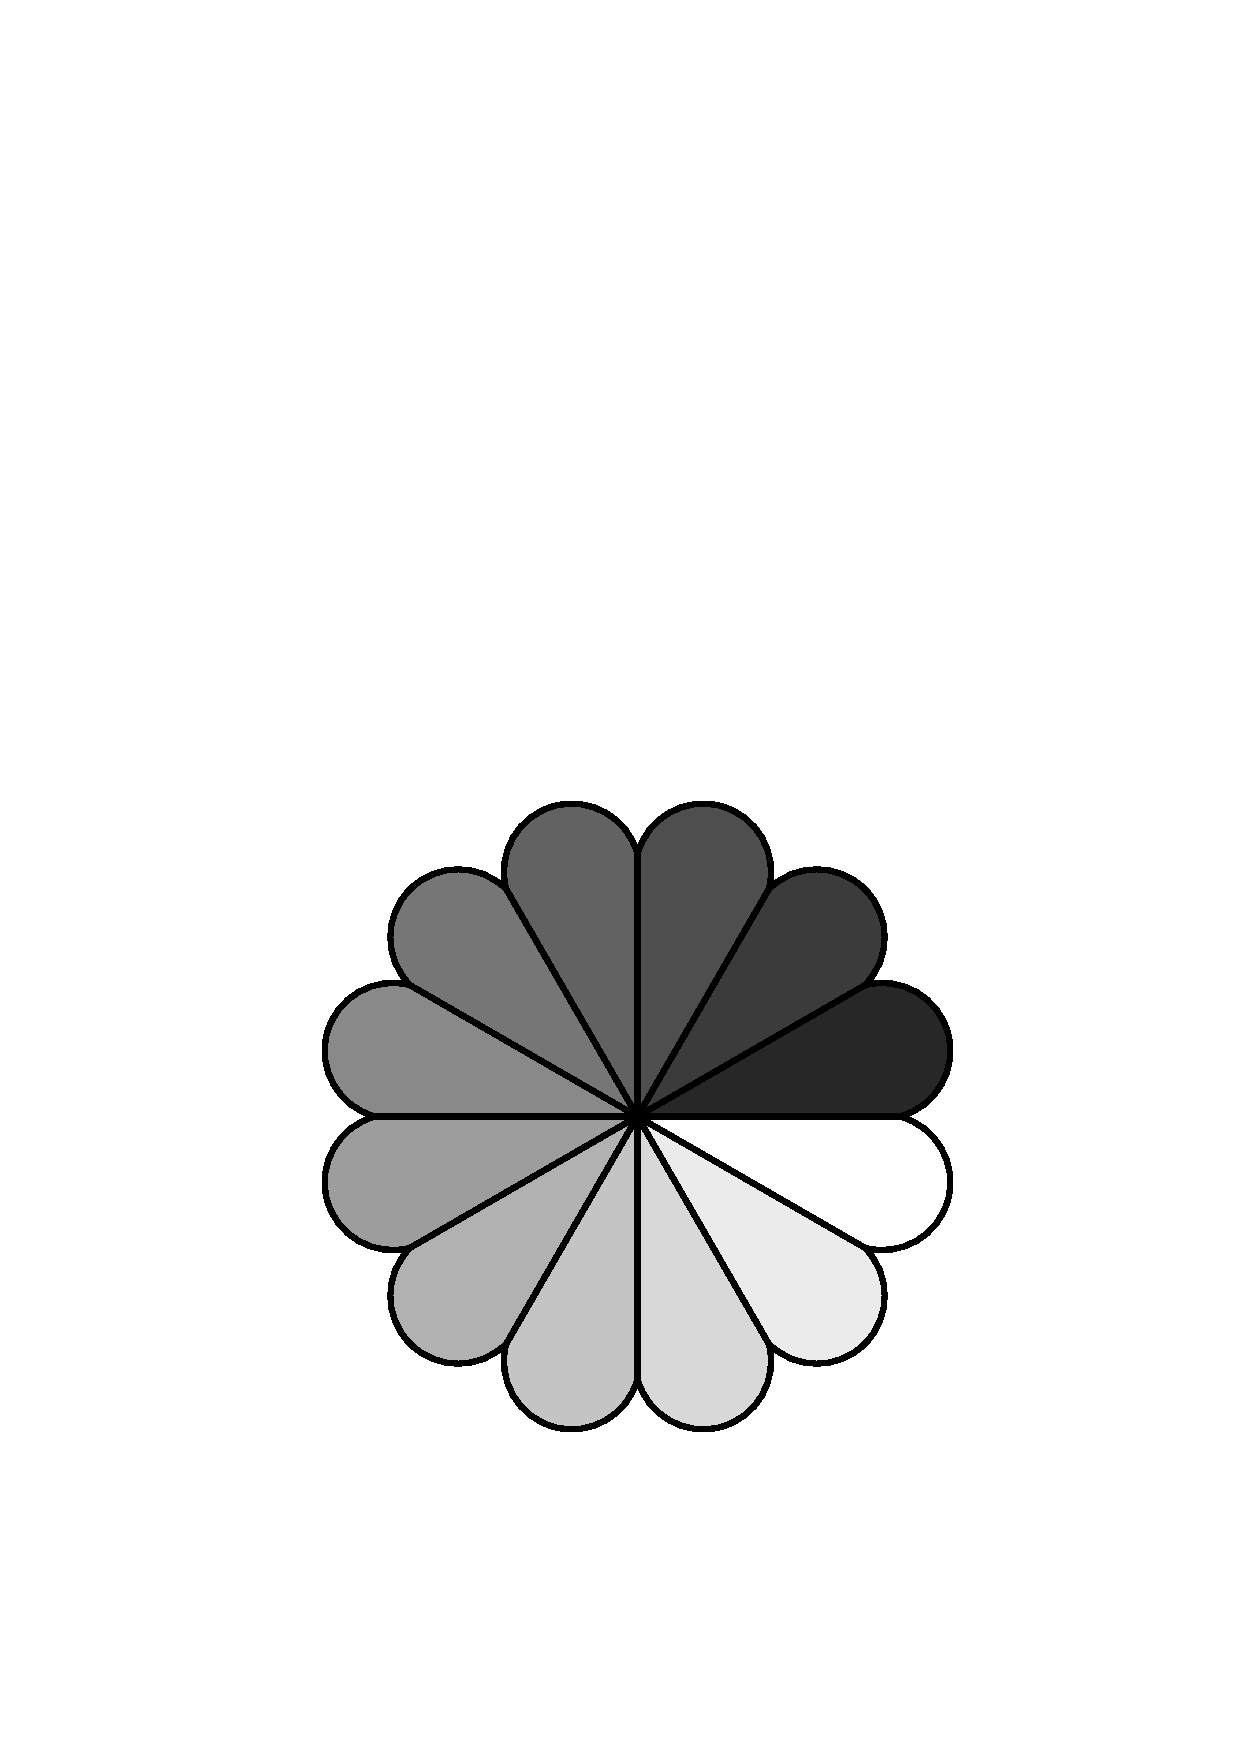
\includegraphics[height=1in, width=1in]{rosette}
\caption{A sample black and white graphic that has
been resized with the \texttt{includegraphics} command.}
\end{figure}

\subsection{Theorem-like Constructs}

Other common constructs that may occur in your article are the forms
for logical constructs like theorems, axioms, corollaries and proofs.
ACM uses two types of these constructs:  theorem-like and
definition-like.

Here is a theorem:
\begin{theorem}
  Let $f$ be continuous on $[a,b]$.  If $G$ is
  an antiderivative for $f$ on $[a,b]$, then
  \begin{displaymath}
    \int^b_af(t)\,dt = G(b) - G(a).
  \end{displaymath}
\end{theorem}

Here is a definition:
\begin{definition}
  If $z$ is irrational, then by $e^z$ we mean the
  unique number that has
  logarithm $z$:
  \begin{displaymath}
    \log e^z = z.
  \end{displaymath}
\end{definition}

The pre-defined theorem-like constructs are \textbf{theorem},
\textbf{conjecture}, \textbf{proposition}, \textbf{lemma} and
\textbf{corollary}.  The pre-defined de\-fi\-ni\-ti\-on-like constructs are
\textbf{example} and \textbf{definition}.  You can add your own
constructs using the \textsl{amsthm} interface~\cite{Amsthm15}.  The
styles used in the \verb|\theoremstyle| command are \textbf{acmplain}
and \textbf{acmdefinition}.

Another construct is \textbf{proof}, for example,

\begin{proof}
  Suppose on the contrary there exists a real number $L$ such that
  \begin{displaymath}
    \lim_{x\rightarrow\infty} \frac{f(x)}{g(x)} = L.
  \end{displaymath}
  Then
  \begin{displaymath}
    l=\lim_{x\rightarrow c} f(x)
    = \lim_{x\rightarrow c}
    \left[ g{x} \cdot \frac{f(x)}{g(x)} \right ]
    = \lim_{x\rightarrow c} g(x) \cdot \lim_{x\rightarrow c}
    \frac{f(x)}{g(x)} = 0\cdot L = 0,
  \end{displaymath}
  which contradicts our assumption that $l\neq 0$.
\end{proof}

\section{Conclusions}
 Provenance collection offers benefits to IoT. It provides trust of data across various layers of the framework. Provenance collection leads to memory. This ensures flexibility in the amount of provenance data stored on the IoT device. It also offers device administrators authority to decide a limit on the amount of provenance data that can be retained ensuring storage efficiency. In this paper, we present a policy-based approach to provenance data pruning. 
%\end{document}  % This is where a 'short' article might terminate



\appendix
%Appendix A
\section{Headings in Appendices}
The rules about hierarchical headings discussed above for
the body of the article are different in the appendices.
In the \textbf{appendix} environment, the command
\textbf{section} is used to
indicate the start of each Appendix, with alphabetic order
designation (i.e., the first is A, the second B, etc.) and
a title (if you include one).  So, if you need
hierarchical structure
\textit{within} an Appendix, start with \textbf{subsection} as the
highest level. Here is an outline of the body of this
document in Appendix-appropriate form:
\subsection{Introduction}
\subsection{The Body of the Paper}
\subsubsection{Type Changes and  Special Characters}
\subsubsection{Math Equations}
\paragraph{Inline (In-text) Equations}
\paragraph{Display Equations}
\subsubsection{Citations}
\subsubsection{Tables}
\subsubsection{Figures}
\subsubsection{Theorem-like Constructs}
\subsubsection*{A Caveat for the \TeX\ Expert}
\subsection{Conclusions}
\subsection{References}
Generated by bibtex from your \texttt{.bib} file.  Run latex,
then bibtex, then latex twice (to resolve references)
to create the \texttt{.bbl} file.  Insert that \texttt{.bbl}
file into the \texttt{.tex} source file and comment out
the command \texttt{{\char'134}thebibliography}.



% This next section command marks the start of
% Appendix B, and does not continue the present hierarchy
\section{More Help for the Hardy}

Of course, reading the source code is always useful.  The file
\path{acmart.pdf} contains both the user guide and the commented
code.

\begin{acks}
  The authors would like to thank Dr. Yuhua Li for providing the
  matlab code of  the \textit{BEPS} method. 

  The authors would also like to thank the anonymous referees for
  their valuable comments and helpful suggestions. The work is
  supported by the \grantsponsor{GS501100001809}{National Natural
    Science Foundation of
    China}{http://dx.doi.org/10.13039/501100001809} under Grant
  No.:~\grantnum{GS501100001809}{61273304}
  and~\grantnum[http://www.nnsf.cn/youngscientsts]{GS501100001809}{Young
    Scientsts' Support Program}.

\end{acks}
